\chapter{Конструкторский раздел}

\section{Модель оценки трудоемкости алгоритмов}
Введем модель оценки трудоемкости.

\begin{enumerate}
	\item Трудоемкость базовых операций.
	Пусть трудоемкость следующих операций равна 2. 
	$$*, /, //, \%, *=, /= $$
	
	Примем трудоемкость следующих операций равной 1.
	$$=, +, -, +=, -=, ==, !=, <, >, <=, >=, |, \&\&, ||, []$$  
	\item Трудоемкость цикла.
	Пусть трудоемкость цикла определяется по формуле (\ref{eq1}).
	
	\begin{equation}
		\label{eq1} 
		f = f_{init} + f_{comp} + N_{iter} * (f_{in} + f_{inc} + f_{comp})
	\end{equation} 
	где:
	\begin{itemize}
		\item $f_{init}$ - трудоемкость инициализации переменной-счетчика;
		\item $f_{comp}$ - трудоемкость сравнения;
		\item $N_{iter}$ - номер выполняемой итерации;
		\item $f_{in}$ - трудоемкость команд из тела цикла;
		\item $f_{inc}$ -трудоемкость инкремента;
		\item $f_{comp}$ - трудоемкость сравнения.
	\end{itemize}
	\item Трудоемкость условного оператора. \\
	Пусть трудоемкость самого условного перехода равна 0, но она определяется по формуле (\ref{eq2}). 
	\begin{equation}
		\label{eq2}
		f_{if} = f_{comp\_if} + \begin{cases}
			f_{a}\\
			f_{b}\\
		\end{cases}
	\end{equation}
	
\end{enumerate}

\section{Вычисление трудоемкости алгоритмов}
Пусть размер массивов во всех дальнейших вычислениях обозначается как N.
\subsection{Трудоемкость алгоритма сортировки пузырьком}
Трудоемкость этого алгоритма сортировки состоит из:

\begin{itemize}
	\item трудоемкость внешнего цикла вычисляется по формуле (\ref{eq3});
	\begin{equation}
		\label{eq3} 
		f_{i} = {\underset{=}{1}} + {\underset{<}{1}} + N= 2 + N
	\end{equation}
	
	\item трудоемкость внутреннего цикла вычисляется по формуле (\ref{eq4}).
	\begin{equation}
		\label{eq4} 
		f_{j} = {\underset{i++}{2}} + {\underset{=}{1}} + {\underset{<}{1}} + {\underset{-}{1}} +
		\frac{N-1}{2}*({\underset{j++}{2}} + f_{if}) = 6 + \frac{N-1}{2}*(2 + f_{if})
	\end{equation}
	
	где вычисление худшего/лучшего случая определяется по формуле (\ref{eq5}):
	\begin{equation}
		\label{eq5}
		f_{if} = {\underset{>}{1}} + {\underset{[\ ]}{2}} + {\underset{+}{1}} +
		\begin{cases}
			0\\
			{\underset{=}{3}} + {\underset{[\ ]}{4}} +{\underset{+}{2}}\\
		\end{cases}
		= 4 +
		\begin{cases}
			0, \text{  лучший случай}\\
			9, \text{  худший случай}
		\end{cases}
	\end{equation}
	
	Трудоемкость пузырька для лучшего случая (\ref{eq7}):
	\begin{equation}
		\label{eq7}
		f_{sum} = 3N^2 + 3N + 2 \approx O(N^2)
	\end{equation}
	
	Трудоемкость пузырька для худшего случая (\ref{eq8}):
	\begin{equation}
		\label{eq8}
		f_{sum} = 7.5N^2 - 1.5N + 2 \approx O(N^2)
	\end{equation}
	
\end{itemize}
\subsection{Трудоемкость алгоритма сортировки простыми вставками}
Трудоемкость этого алгоритма сортировки состоит из:
\begin{itemize}
	\item трудоемкость внешнего цикла вычисляется по формуле (\ref{eq9});
	\begin{equation}
		\label{eq9}
		f_{i} = {\underset{=}{1}} + {\underset{<}{1}} + N= 2 + N
	\end{equation}
	
	\item трудоемкость тела внутреннего цикла определяется по формуле (\ref{eq10}).
	\begin{equation}
		\label{eq10} 
		f_{body} = {\underset{i++}{2}} + {\underset{=}{2}} + {\underset{[\ ]}{1}} + {\underset{-}{1}} + f_{if} + {\underset{[\ ]}{1}} + {\underset{+}{1}} + {\underset{=}{1}}
	\end{equation}
	
	где $f_{if}$ вычисляется по формуле (\ref{eq11}):
	\begin{equation}
		\label{eq11}
		f_{if} = {\underset{>=}{1}} + {\underset{\&\&}{1}} + {\underset{<}{1}} + {\underset{[\ ]}{1}} +
		\begin{cases}
			0\\
			{\underset{=}{3}} + {\underset{[\ ]}{4}} +{\underset{+}{2}}\\
		\end{cases}
		= 4 +
		\begin{cases}
			0, \text{  лучший случай}\\
			\frac{N-1}{4} * ({\underset{[\ ]}{2}} + {\underset{+}{1}} + {\underset{-=}{1}} + {\underset{=}{1}}),\\
			\text{  худший случай}
		\end{cases}
	\end{equation}
	
	Трудоемкость алгоритма сортировки простыми вставками для лучшего случая (\ref{eq12}):
	\begin{equation}
		\label{eq12}
		f_{sum} = 13N + 2 \approx O(N)
	\end{equation}
	
	Трудоемкость алгоритма сортировки простыми вставками для худшего случая (\ref{eq13}):
	\begin{equation}
		\label{eq13}
		f_{sum} = \frac{5N^2}{4} - \frac{47N}{4} + 2 \approx O(N^2)
	\end{equation}
\end{itemize}

\subsection{Трудоемкость алгоритма сортировки методом Шелла}
Пусть шаг в методе Шелла будет равен N/2, где N - размер массива. Трудоемкость этого алгоритма сортировки состоит из:
\begin{itemize}
	\item трудоемкость внешнего цикла вычисляется по формуле (\ref{eq14});
	\begin{equation}
		\label{eq14}
		f_{i} = {\underset{//=}{2}} + {\underset{=}{1}} + {\underset{<}{1}} +  
		{\underset{i++}{2}} + {\underset{=}{1}} +  \frac{N}{2} * ({\underset{i++}{2}} + {\underset{=}{1}} + {\underset{>=}{1}} + {\underset{[\ ]}{2}} + {\underset{>}{1}} + {\underset{+}{1}} + {\underset{\&\&}{1}} + \frac{N}{2} (f_{if}))
	\end{equation}
	\item трудоемкость $f_{if}$ вычисляется по формуле (\ref{eq15}).
	\begin{equation}
		\label{eq15}
		f_{if} = {\underset{=}{3}} + {\underset{[\ ]}{4}} + {\underset{+}{2}} + {\underset{-=}{1}}
	\end{equation}
	
	Трудоемкость алгоритма сортировки методом Шелла для лучшего случая (\ref{eq16}):
	\begin{equation}
		\label{eq16}
		f_{sum} = \frac{9N}{2} + 7 \approx O(N)
	\end{equation}
	
	Трудоемкость алгоритма сортировки методом Шелла для худшего случая (\ref{eq17}):
	\begin{equation}
		\label{eq17}
		f_{sum} = \frac{10N^2}{4} + \frac{9N}{2} + 7 \approx O(N^2)
	\end{equation}
\end{itemize}

\section{Схемы алгоритмов сортировок}
Ниже представлены следующие схемы алгоритмов:
\newpage
\begin{itemize}
	\item рис. \ref{png:1} - схема алгоритма сортировки пузырьком;
	\begin{figure}[H]
		\centering{
			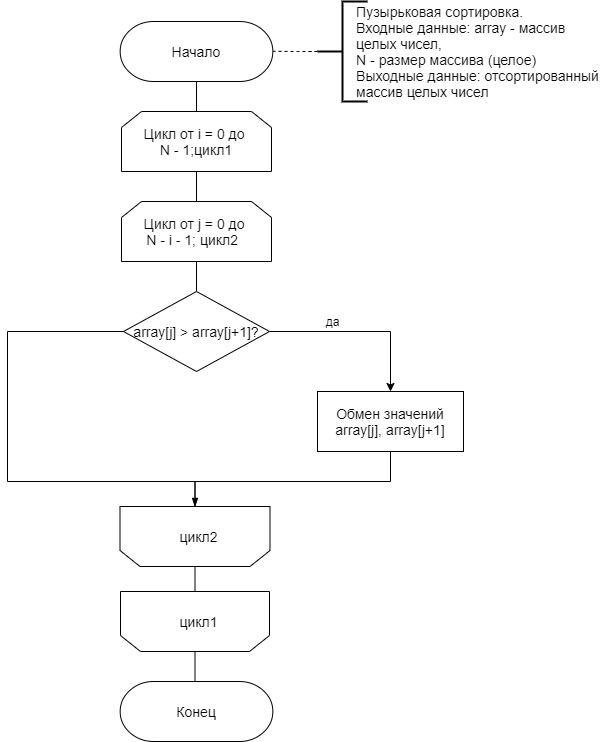
\includegraphics[scale=0.7]{../../../../../../../msys64/home/Лев/bmstu_sem_5_aa/lab_03/report/diagrams/bubble}
			\caption{Схема алгоритма сортировки пузырьком.}
			\label{png:1}}
	\end{figure} 
	
	\newpage
	\item рис. \ref{png:2} - схема алгоритма сортировки простыми вставками;
	\begin{figure}[H]
		\centering{
			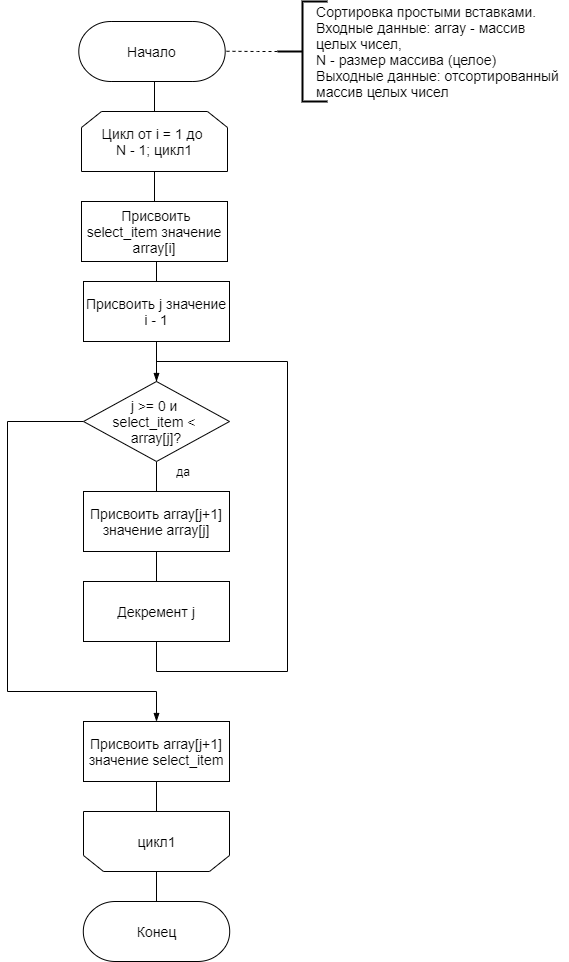
\includegraphics[scale=0.6]{../../../../../../../msys64/home/Лев/bmstu_sem_5_aa/lab_03/report/diagrams/insert}
			\caption{Схема алгоритма сортировки простыми вставками.}
			\label{png:2}}
	\end{figure} 
	
	\newpage
	\item рис. \ref{png:3} - схема алгоритма сортировки методом Шелла.
	\begin{figure}[H]
		\centering{
			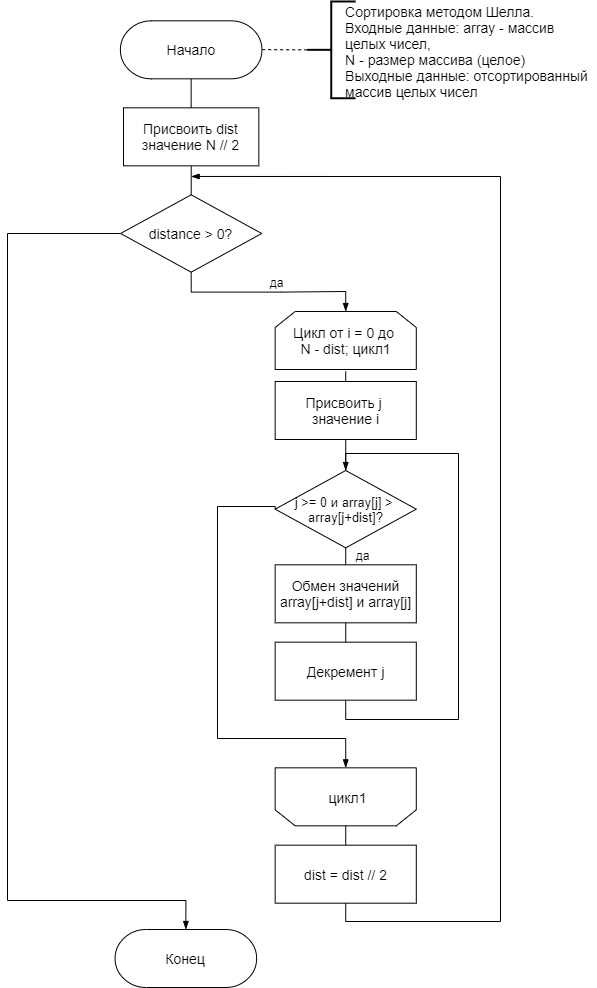
\includegraphics[scale=0.6]{../../../../../../../msys64/home/Лев/bmstu_sem_5_aa/lab_03/report/diagrams/shell}
			\caption{Cхема алгоритма сортировки методом Шелла.}
			\label{png:3}}
	\end{figure}
\end{itemize}

\section{Вывод}
На основе теоретических данных, полученных в аналатическом разделе, были построены схемы нужных алгоритмов. Были получена трудоемкость каждого из трех алгоритмов для анализа худшего и лучшего случаев асимптотической сложности. Полученная трудоемкость приведена в таблице \ref{table:ref1}:

\begin{table}[ht!]
	\centering
	\captionsetup{singlelinecheck = false, justification=raggedleft}
	\caption{Сложность алгоритмов.}
	\label{table:ref1}
	\begin{tabular}{|c|c|c|}
		\hline
		\multirow{2}{*}{Алгоритм}& \multicolumn{2}{c|}{Сложность} \\ \cline{2-3} 
		                         & Лучший случай & Худший случай \\
		\hline
		Пузырек & $O(N^2)$  & $O(N^2)$ \\
		\hline
		Простые вставки & $O(N)$  & $O(N^2)$ \\
		\hline
		Шелл & $O(N)$  & $O(N^2)$ \\
		\hline
	\end{tabular}
\end{table}